\documentclass{estilo}
\usepackage[spanish]{babel}
\usepackage{graphicx}
\usepackage{float}
\usepackage{amsmath}        % para los vectores columnas
\usepackage{amsfonts}       % para las negrita de pizarra
\usepackage{amssymb}        % para simbolos matematicos
\usepackage{hyperref}       % para utilizar referencias

\usepackage[style=authoryear-comp]{biblatex}

\begin{document}
\maketitle

\section*{Enunciado}
Los datos del archivo \textit{cemento.txt} fueron tomados en un estudio experimental para relacionar el calor generado (Y) al fraguar 14 muestras de cemento con distinta composición. Las variables explicativas son los pesos (medidos en porcentajes del peso de cada muestra de cemento) de 5 componentes del cemento.

\begin{enumerate}
    \item[\hyperlink{ej1}{1.}] Calcular la matriz de correlación de todas las variables comprendidas en el problema, incluyendo a la variable Y. Inspeccionando esta matriz determinar cuáles parecen ser las variables que pueden contribuir significativamente a explicar la variación de Y.
    \item[\hyperlink{ej2}{2.}] Usar Y como variable dependiente y todas las covariables y una intercept para realizar un ajuste lineal. Calcular el estimador de mínimos cuadrados de los parámetros y para cada uno de ellos testear la hipótesis de que es 0. ¿Cuáles son significativamente distintos de 0? ¿es la regresión significativa? ¿Observa alguna contradicción con el resultado obtenido en los tests individuales anteriores? ¿Vale la pena hacer un nuevo intento para seleccionar qué variables entran en la regresión?
    \item[\hyperlink{ej3}{3.}] Calcular la suma de las 5 covariables. ¿Qué observa? ¿Cómo se justifica este parecido entre los totales? A partir de este resultado, ¿Puede justificar esto que eliminemos del modelo la intercept?
    \item[\hyperlink{ej4}{4.}] Realizar un nuevo ajuste lineal usando las 5 variables independientes y eliminando la intercept. ¿Cómo se comparan estos resultados con los obtenidos anteriormente? ¿Cuáles son significativamente distintos de 0?
    \item[\hyperlink{ej5}{5.}] Plantear un nuevo modelo en el que intervengan aquellas variables que contribuyen significativamente y estimar los parámetros por mínimos cuadrados. ¿Qué modelo elegiría finalmente?
    \item[\hyperlink{ej6}{6.}] A partir de la estimación del error cuadrático medio, determinar si de todos los modelos planteados en el ejercicio, el seleccionado en el ítem anterior parece ser el mejor.
\end{enumerate}
\newpage

\section*{Marco teórico}
\subsection*{Coeficiente de correlación de Pearson}
Dadas X e Y variables aleatorias, el coeficiente de correlación de Pearson entre X e Y está definido como:

\begin{minipage}{\linewidth}
  \centering
  \begin{minipage}{0.45\linewidth}
    $$\rho_{_{X,Y}} = \frac{Cov(X, Y)}{\sqrt{Var(X) \cdot Var(Y)}}$$
  \end{minipage}
  \hspace{0.05\linewidth}
  \begin{minipage}{0.45\linewidth}
    $$-1 \leq \rho_{_{X,Y}} \leq 1$$
  \end{minipage}
\end{minipage}

Siendo:
$$Cov(X,Y) \dot{=} E[(X - E[X]) \cdot (Y - E[Y])]$$

Dado que no conocemos la distribución de las variables, necesitamos una estimación de $\rho_{_{X,Y}}$. Por lo que utilizaremos:

$$\hat{\rho}_{_{X,Y}} = \frac{\sum\limits_{i=1}^{n} (x_i - \bar{x})(y_i - \bar{y})} {\sqrt{\sum\limits_{i=1}^{n}(x_i - \bar{x})^2} \sqrt{\sum\limits_{i=1}^{n}(y_i - \bar{y})^2}}$$
donde, $\bar{x}$ es el promedio de los valores observados. Y se utiliza el estimador de máxima verosimilitud para el desvío.

\subsection*{Modelo $\Omega$}
Se tienen $n$ observaciones del vector aleatorio $(X_{1}, X_{2}, ..., X_{p-1}, Y)$, se propone, bajo los supuestos necesarios, el siguiente modelo:
$$Y = \beta_{0} + \beta_{1} \cdot x_{1} + ... + \beta_{p-1} \cdot x_{p-1} + \epsilon$$
De forma que, para cada observación se tiene:
$$y_i = \beta_{0} + \beta_{1} \cdot x_{i,1} + ... + \beta_{p-1} \cdot x_{i, p-1} + \epsilon_{i} \quad  \forall i = 1,..,n$$
Con $\epsilon_{i}$ variables aleatorias no observables.\\

\textbf{Supuestos}
\begin{enumerate}
    \item $E[\epsilon_{i}] = 0$
    \item $Var(\epsilon_{i}) = \sigma^2$
    \item $\epsilon_{i} \stackrel{iid}{\sim} \mathcal{N}(0, \sigma^2)$
\end{enumerate}

\textbf{Expresiones}
De ahora en adelante $X$ será fijo en $x$.

\begin{minipage}{\linewidth}
  \centering
  \begin{minipage}{0.10\linewidth}
        \begin{align*}
            Y &= \begin{bmatrix}
            y_{1} \\
            y_{2} \\
            \vdots \\
            y_{n}
            \end{bmatrix}
        \end{align*}
  \end{minipage}
  \hspace{0.05\linewidth}
  \begin{minipage}{0.10\linewidth}
        \begin{align*}
            \epsilon &= \begin{bmatrix}
            \epsilon_{1} \\
            \epsilon_{2} \\
            \vdots \\
            \epsilon_{n}
            \end{bmatrix}
        \end{align*}
  \end{minipage}
  \hspace{0.05\linewidth}
  \begin{minipage}{0.10\linewidth}
        \begin{align*}
            \beta &= \begin{bmatrix}
            \beta_{0} \\
            \beta_{1} \\
            \vdots \\
            \beta_{p-1}
            \end{bmatrix}
        \end{align*}
  \end{minipage}
  \hspace{0.05\linewidth}
  \begin{minipage}{0.40\linewidth}
        \begin{align*}
            \mathbb X &= \begin{bmatrix}
            1 & x_{1,1}  & \dots & x_{1, p-1} \\
            1 & x_{2,1}  & \dots & x_{2, p-1} \\
            \vdots & \vdots & \ddots & \vdots \\
            1 & x_{n,1} & \dots & x_{n, p-1} \\
            \end{bmatrix}
        \end{align*}
  \end{minipage}
\end{minipage}
\vskip0.5cm
Por lo tanto, se tiene que:
$$Y = \mathbb X \beta + \epsilon$$
Y, si $\mathbb X$ tiene rango completo, entonces se deducen las siguientes expresiones

$$ \hat{\beta} = ({\mathbb X}^T \mathbb X)^{-1} {\mathbb X}^T Y$$
$$ \hat{Y} = \mathbb X ({\mathbb X}^T \mathbb X)^{-1}{\mathbb X}^T Y = P Y$$

Por último, se define como \textbf{residuo} a $r = Y - \hat{Y}$

\subsection*{Test de hipótesis}
Bajo el modelo $\Omega$: los estimadores $\hat{\beta}$ y $S^{2}$ son IMVU (\textbf{I}nsesgado de \textbf{M}ínima \textbf{V}arianza \textbf{U}niformemente)

\vskip0.4cm
\textbf{Test t}
\vskip0.2cm
\begin{minipage}{\linewidth}
  \begin{minipage}{0.40\linewidth}
    \centering
    $H_0: \beta_{i} = 0$
  \end{minipage}
  \hspace{0.05\linewidth}
  \begin{minipage}{0.05\linewidth}
    \centering vs
  \end{minipage}
  \hspace{0.05\linewidth}
  \begin{minipage}{0.40\linewidth}
    \centering
    $H_1: \beta_{i} \neq 0$
  \end{minipage}
\end{minipage}
\vskip0.2cm
Sabiendo que $\hat{\beta_{i}} \sim \mathcal{N}(\beta_{i}, \sigma^2 D_{i,i})$ se obtiene el estadístico $T$ de la siguiente forma:
$$
T = \frac{\hat{\beta_{i}} - \beta_{i}}{S \sqrt{D_{i,i}}}
$$
siendo $D_{i,i}$ el elemento $i$ de la diagonal de la matriz $({\mathbb X}^{T} \mathbb X)^{-1}$\\
\vskip0.2cm
\begin{minipage}{\linewidth}
  \begin{minipage}{0.55\linewidth}
    \begin{figure}[H]
        \centering
        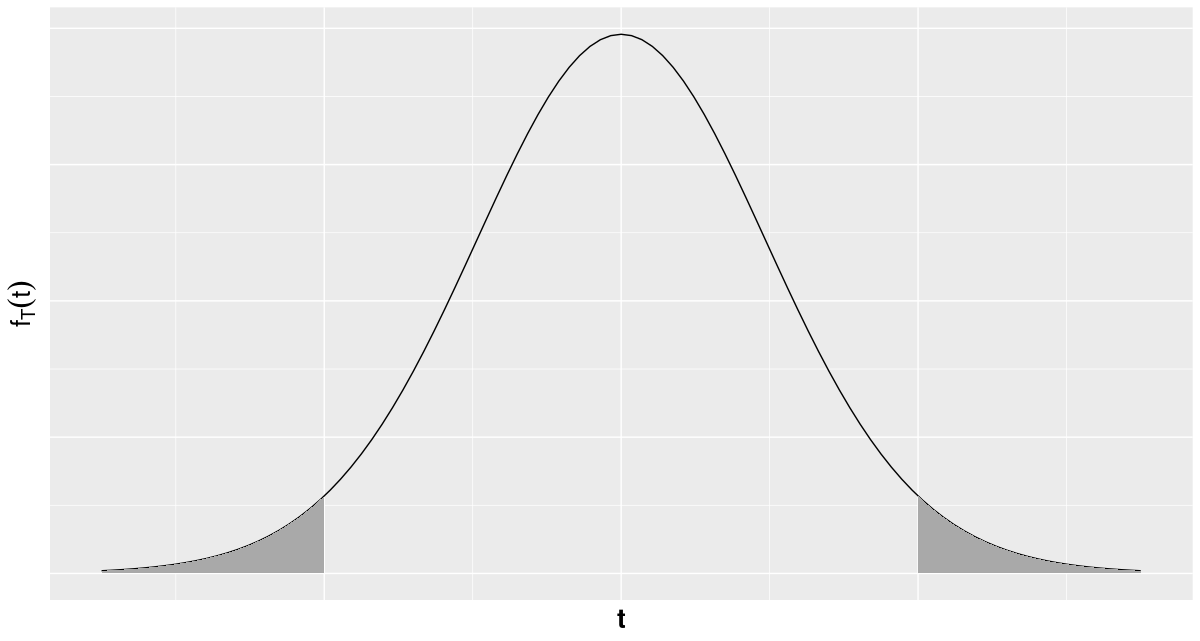
\includegraphics[width=1\textwidth]{resources/t_student_density.png}
        \caption{Densidad de T bajo $H_0$}
    \end{figure}
  \end{minipage}
  \hspace{0.05\linewidth}
  \begin{minipage}{0.35\linewidth}
        De forma que bajo $H_0$ se tiene que 
        $$T \sim t_{n-p}$$
        Por lo que, se calculará el p-valor como el area sombreada en la figura
        $$ p-value = P(|T| > t_{obs})$$
  \end{minipage}
\end{minipage}
\vskip0.4cm
\textbf{Test F}
\vskip0.2cm
\begin{minipage}{\linewidth}
  \begin{minipage}{0.40\linewidth}
    \centering
    $H_0: \beta_{1} = ... = \beta_{p-1} = 0$
  \end{minipage}
  \hspace{0.05\linewidth}
  \begin{minipage}{0.05\linewidth}
    \centering vs
  \end{minipage}
  \hspace{0.05\linewidth}
  \begin{minipage}{0.40\linewidth}
    \centering
    $H_1:$ Algún $\beta_{i} \neq 0$
  \end{minipage}
\end{minipage}
\vskip0.2cm

El estadístico a utilizar para este Test será $F$, cuya expresión será la siguiente
$$
F = \frac{(C\hat{\beta})^{T} (C ({\mathbb X}^T \mathbb X)^{-1} {C}^{T})^{-1}(C \hat{\beta})}{(p-1) S^{2}} \stackrel{H_0}{\sim} {\mathcal F}_{p-1, n-p}
$$
siendo
\begin{align*}
    C &= \begin{bmatrix}
    0 & 1 & 0 & \dots & 0 \\
    0 & 0 & 1 & \dots & 0 \\
    \vdots & \vdots & \vdots & \ddots & \vdots \\
    0 & 0 & 0 & \dots & 1 \\
    \end{bmatrix} \in \mathbb R ^{(p-1) \times p}, \quad rg(C) = p-1
\end{align*}

\vskip0.2cm
\begin{minipage}{\linewidth}
  \begin{minipage}{0.55\linewidth}
    \begin{figure}[H]
        \centering
        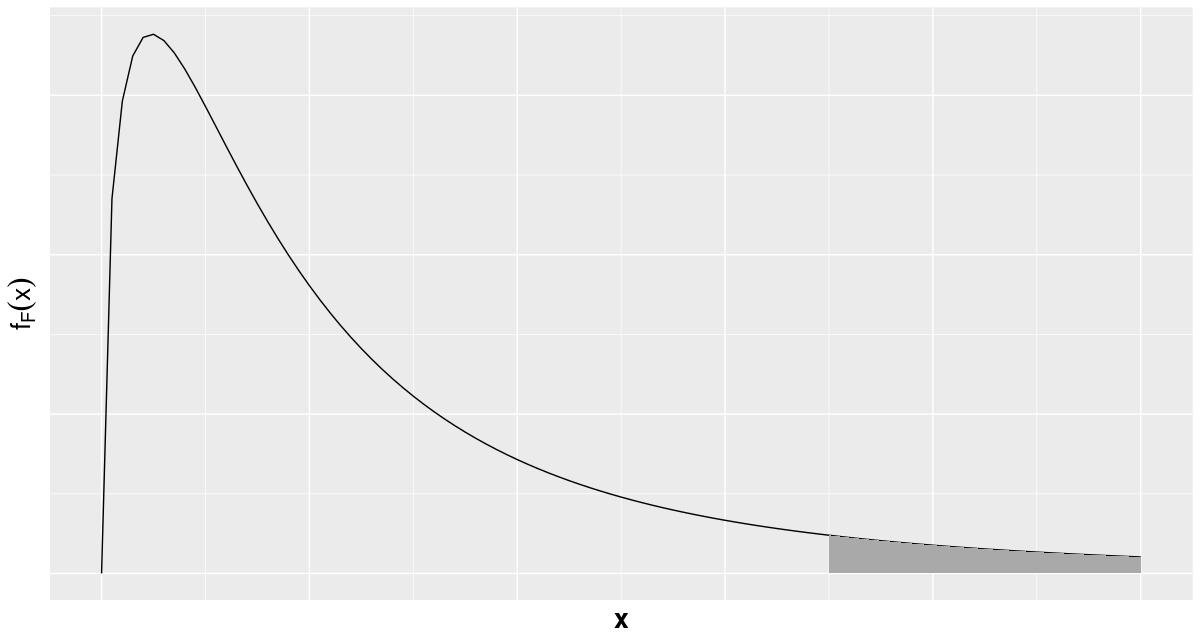
\includegraphics[width=1\textwidth]{resources/f_fisher_density.png}
        \caption{Densidad de F bajo $H_0$}
    \end{figure}
  \end{minipage}
  \hspace{0.05\linewidth}
  \begin{minipage}{0.35\linewidth}
        Por lo que, se calculará el p-valor como el area sombreada en la figura
        $$ p-value = P(F > x_{obs})$$
  \end{minipage}
\end{minipage}
\vskip0.4cm
\textbf{Observación:} a lo largo del trabajo práctico tomaremos un nivel de significancia mínimo $\alpha = 0.05$ de forma que para cualquier p-valor menor a $\alpha$ rechazaremos siempre la hipótesis nula.

\subsection*{Selección de variables}
En el trabajo práctico utilizaremos el método de selección \textbf{StepWise: forward} una heurística greedy que analiza los modelos desde el más simple (sólo 1 variable predictora) hasta el más complejo (todas las variables predictoras) de forma incremental. Su método de selección se basa en el test F: irá seleccionando las variables predictoras en base al modelo que obtenga un estadístico F mayor.

\subsection*{Análisis de residuos}
Los residuos, previamente definidos como $r_i = y_i - \hat{y}_{i}$ serán variables aleatorias con:
\begin{center}
    \begin{itemize}
        \item $E[r_i] = 0$
        \item $Var[r_i] = {\sigma}^2(1-P_{i,i})$
    \end{itemize}
\end{center}
Asumiendo que siguen una distribución normal se tiene que:
$$
\frac{r_i}{\sqrt{\sigma^2 (1-P_{i,i})}} \sim \mathcal{N}(0, 1)
$$
Pero como desconocemos el valor de $\sigma^2$ se utilizarán los \textbf{residuos studentizados}, que se definen de la siguiente manera:
$$
t_i = \frac{r_i}{\sqrt{S^2(1-P_{i,i})}}
$$
tal que si $r_i$ llevan una distribución normal los $t_i$ tendrán distribución t-student.
\vskip0.2cm\textbf{Comparación según error cuadrático medio}\\
Para realizar comparaciones basadas en el ECM (Error Cuadrático Medio) que no subestimen el valor obtenido se utilizarán los residuos de LOOCV (Leave One Out Cross Validation), que consisten en, para un mismo modelo, realizar la regresión para todas las observaciones en la muestra menos 1.\\
Se definen entonces los residuos de validación cruzada como:
$$
r_{-i} =  = y_{i} - \hat{\beta}_{-i} x_i
$$
siendo $\hat{\beta}_{-i}$ los coeficientes obtenidos de la regresión sin tener en cuenta la observación $i$.\\
Este residuo se calculará de manera equivalente con la siguiente expresión:
$$
r_{-i} = \frac{r_i}{1-P_{i,i}}
$$
Y se definirá en base a este último lo que llamaremos $ECM_{VC}$ (Error cuadrático medio de validación cruzada)
$$
EMC_{VC} = \frac{1}{n} \sum^{n}_{i=1}(r_{-i})^2
$$
\newpage
\section*{Resolución}
\hypertarget{ej1}{\subsection*{Ejercicio 1}}
A continuación mostramos un pairplot de las variables.

\begin{figure}[H]
    \centering
    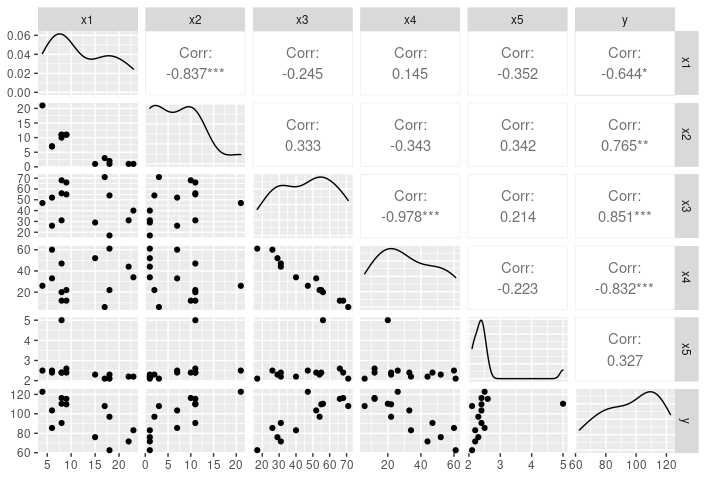
\includegraphics[width=1\textwidth]{resources/GGPairs.png}
    \caption{Pair Plot de las variables}
\end{figure}

\subsubsection*{Análisis general de coeficientes}
En el siguiente gráfico podremos ver con mayor facilidad los coeficientes que dieron significativamente altos entre las covariables. 

\begin{figure}[H]
    \centering
    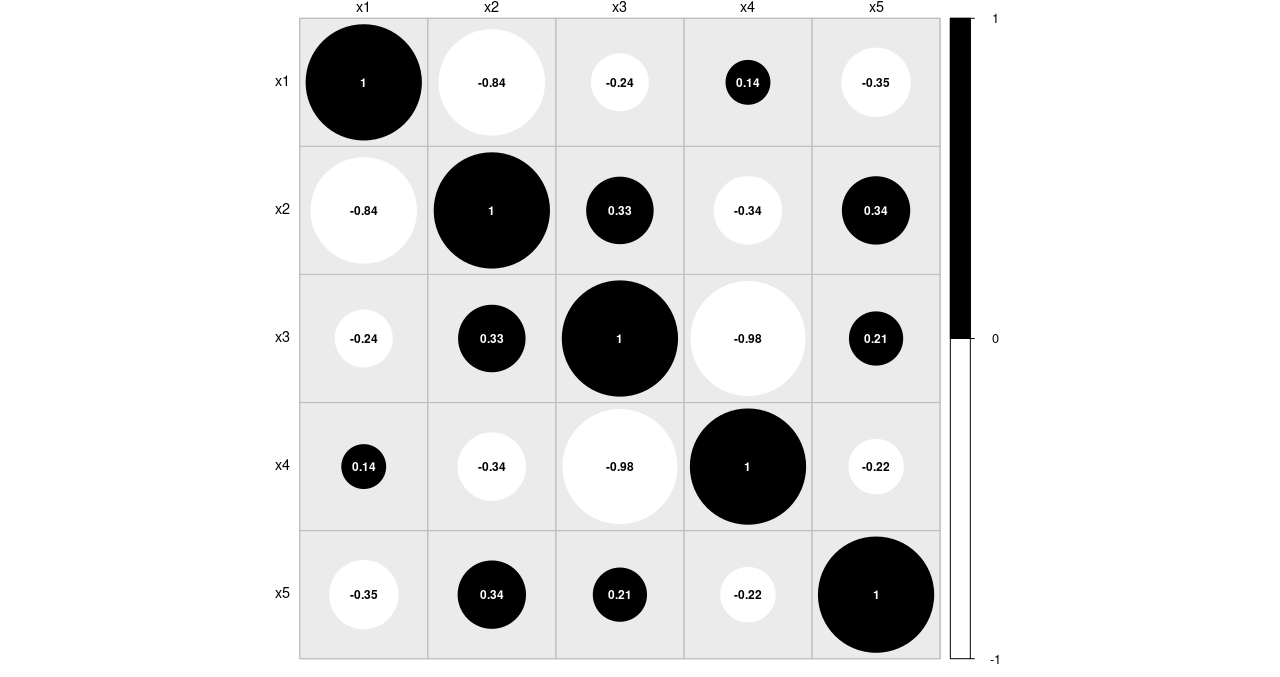
\includegraphics[width=0.8\textwidth]{resources/HeatMapRho.png}
    \caption{Se observa que algunas variables presentan un alto coeficiente de correlación.}
\end{figure}
Los coeficientes entre las covariables y la variable a predecir se verán más adelante.
\vskip0.2cm\textbf{X3 vs X4}\\
Lo primero que destacamos del gráfico es la correlación entre las variables $X_{3}$ y $X_{4}$, dado que se acerca mucho a -1 ($\hat{\rho}_{_{X_{3},X_{4}}} = -0.978$). Esto se corresponde con el gráfico de dispersión entre estas variables, cuyo gráfico se encuentra en la parte inferior de la matriz, y destacamos a continuación.

\begin{figure}[H]
    \centering
    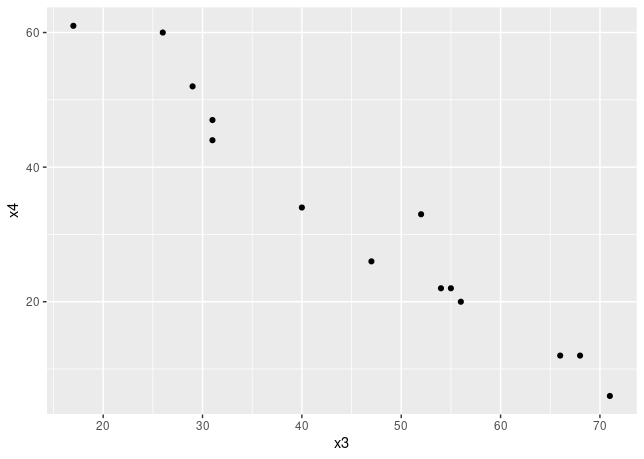
\includegraphics[width=0.8\textwidth]{resources/X3vsX4.png}
    \caption{Gráfico de dispersión entre x3 y x4}
\end{figure}

Viendo este gráfico podemos observar que a medida que aumenta $X_3$, tiende a disminuir $X_4$.\\
Esto nos informa que parece haber una relación lineal muy fuerte entre las variables $X_3$ y $X_4$, situación que habrá que tener en cuenta a la hora de realizar la regresión lineal sobre la variable objetivo ($Y$).
Asimismo, además, podemos observar en el gráfico que las correlaciones entre las diferentes variables con $X_3$ y con $X_4$, en modulo, se parecen.
Por ejemplo, $\hat{\rho}_{_{X_{3},Y}} = 0.851$ y $\hat{\rho}_{_{X_{4},Y}} = -0.832$

\subsubsection*{Valores atípicos}
Pudimos advertir la presencia de valores atípicos en los datos observando sobretodo la fila de la variable $X_5$ y la columna de la variable $X_2$ cuyos valores representaremos en el siguiente gráfico con un boxplot:

\begin{figure}[H]
    \centering
    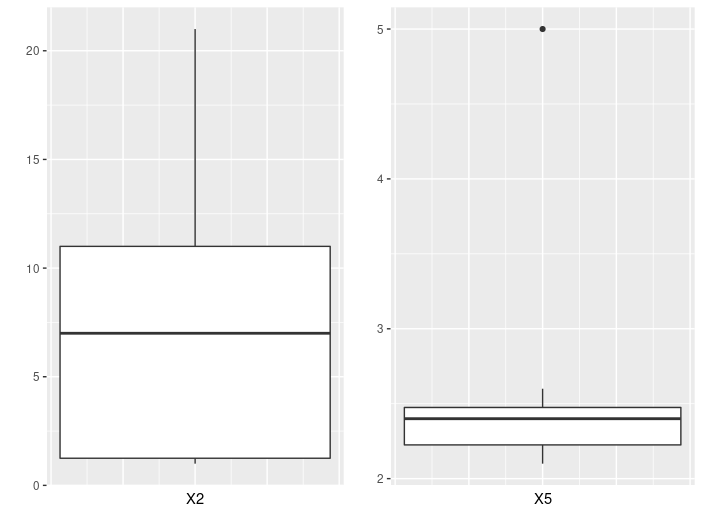
\includegraphics[width=0.6\textwidth]{resources/boxplots_X2_X5.png}
    \label{fig:my_label}
\end{figure}

Desde ya, no podemos descartar estos puntos a pesar de que sean valores atípicos. Sin embargo, debemos prestarles especial atención a la hora de analizar la muestra y más aún al generar nuestro modelo.

\subsubsection*{Relación con la variable objetivo}

\begin{figure}[H]
    \centering
    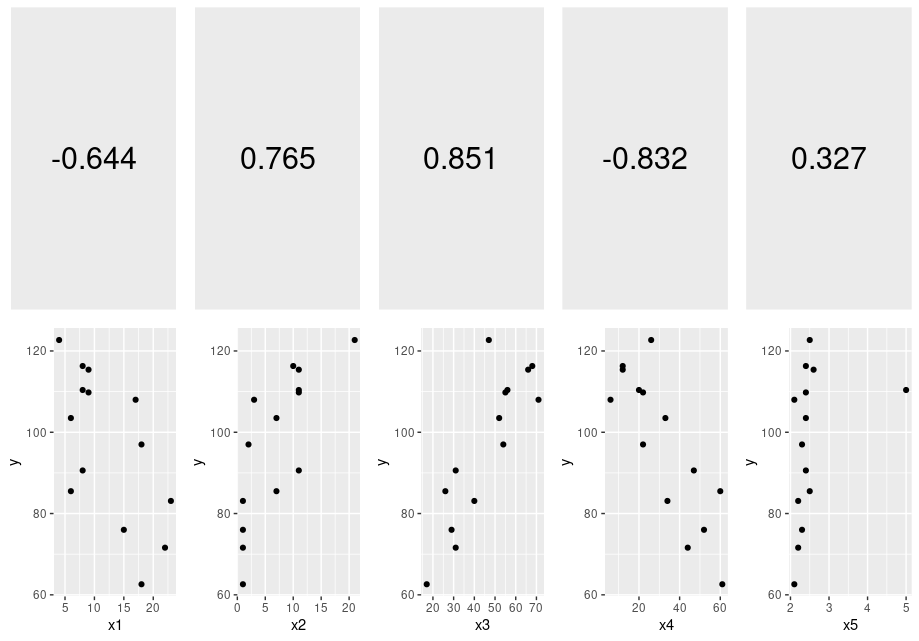
\includegraphics[width=1\textwidth]{resources/x_vs_y.png}
    \caption{Relación entre las variables x y la variable y}
\end{figure}

Podemos ver que a priori, las variables con mayor coeficiente de correlación con Y son X2, X3 y X4 siendo estas dos últimas las de mayor coeficiente.\\
Esto nos servirá como una primera impresión sobre cuáles variables tendrán, a priori, un impacto sobre la variable objetivo.\\
\textbf{Obs:} vemos por ejemplo que la variable X5 tiene un coeficiente de correlación muy bajo, pero cabe destacar que presenta un valor atípico que podría estar provocando que obtengamos una idea errónea sobre su impacto.

\hypertarget{ej2}{\subsection*{Ejercicio 2}}
\textbf{Estimación de los coeficientes y test nulo}

Calculamos el estimador de mínimos cuadrados para los coeficientes, expresándolos en 2 decimales significativos. Para cada uno de estos testeamos la hipótesis de que son nulos, obteniendo para cada coeficiente su correspondiente p-valor. Vale mencionar que para el parámetro $\beta_0$, el intercept, no calculamos su p-valor, dado que suponemos que este existe siempre.

\begin{center}
    \begin{tabular}{|c|c|c|c|}
        \hline
        Coeficiente & Estimación & Rechazo & P-valor \\ \hline
        $\beta_0$ & $73.61$ & - & - \\ \hline
        $\beta_1$ & $-0.45$ & No & $0.701$ \\ \hline
        $\beta_2$ & $1.30$ &  No & $ 0.258$ \\ \hline
        $\beta_3$ & $0.56$ & No & $0.609$ \\ \hline
        $\beta_4$ & $-0.17$ & No & $0.875$ \\ \hline
        $\beta_5$ & $-0.39$ & No & $0.806$ \\ \hline
    \end{tabular}
\end{center}

Podemos ver aquí que ninguno es significativamente distinto de cero, pues los p-valores del test dieron muy alto. Esto quiere decir, que no tenemos pruebas suficientes y por lo tanto no podemos rechazar la hipótesis nula.

\vskip0.2cm\textbf{Significancia de la regresión}\\
Tenemos pruebas suficientes para decir que la regresión utilizada (aquella que utiliza todas las x) es mucho mejor que utilizar sólo la media de la variable objetivo.\\
Esta información la brinda el p-valor del test F, cuyo valor es $p-valor = 2.48 \times 10^{-7}$.
Luego, otra medida que nos brinda información acerca de la significancia de la regresión es el $R^2_{adj} = 0.979$. Esto quiere decir que la regresión sirve para explicar la variabilidad de la variable objetivo adecuadamente.\\

\vskip0.2cm\textbf{Observaciones}\\
Nos llamó la atención que, por más que ninguno de los coeficientes tuvo la significancia suficiente para rechazar la hipótesis nula del test nulo, la significancia final de la regresión dio alta.\\
Esto muy probablemente se deba a que muchas de las variables están altamente correlacionadas; y por lo tanto la varianza para cada uno de los parámetros es muy alta provocando que los intervalos de confianza para los mismos sea muy grande y posiblemente incluya al cero dentro de este.
\vskip0.2cm
Esto nos invita a revisar el modelo propuesto en búsqueda de una selección más adecuada de las variables predictoras.

\vskip0.2cm\textbf{Modelo}\\
\begin{equation}\tag{M1}
    Y = 73.61 -0.45 X_{1} + 1.30 X_{2} + 0.56 X_{3} -0.17 X_{4} -0.39 X_{5}
\end{equation}
\hypertarget{ej3}{\subsection*{Ejercicio 3}}

A continuación calcularemos la suma de las variables predictoras.
\vskip0.1cm
\begin{minipage}{\linewidth}
  \hspace{0.10\linewidth}
      \begin{minipage}{0.20\linewidth}
        \begin{tabular}{| c | c |}
            \hline
            Muestra & Suma \\ \hline
            1 & 101.5 \\ \hline
            2 & 99.3 \\ \hline
            3 & 100.0 \\ \hline 
            4 & 99.4 \\ \hline
            5 & 100.4 \\ \hline
            6 & 99.4 \\ \hline
            7 & 99.1 \\ \hline
            8 & 100.2 \\ \hline
            9 & 98.3 \\ \hline
            10 & 100.5 \\ \hline
            11 & 100.2 \\ \hline
            12 & 100.6 \\ \hline
            13 & 100.4 \\ \hline
            14 & 99.1 \\ \hline
        \end{tabular}
    \end{minipage}
  \hspace{0.05\linewidth}
  \begin{minipage}{0.50\linewidth}
    \justify
    Como es esperado, siendo que cada una de las variables explicativas representan un porcentaje sobre el peso de cada muestra de cemento, las sumas se acercan mucho a 100.\\
    Esto nos indica que las columnas de la matriz de diseño pueden traer consigo un problema: las columnas tienden a ser linealmente dependientes, pues, con algún error asociado, se cumple que $X_1 + X_2 + X_3 + X_4 + X_5 = 100$.\\
        \begin{center}
            \begin{tabular}{| c | c | c | c |}
                \hline
                Min & Max & Mean & Std. Error \\ \hline
                98.30 & 101.50 & 99.89 & 0.82 \\ \hline
            \end{tabular}       
        \end{center}
  \end{minipage}
\end{minipage}
\vskip0.2cm
Por lo tanto, respecto a la pregunta de si tiene sentido eliminar el intercept de la regresión:\\
Teóricamente el hecho de que las columnas de la matriz de diseño sean linealmente dependientes nos indica que el modelo tendrá el mismo error cuadrático medio si reducimos en uno la cantidad de parámetros. Sin pérdida de generalidad, mostramos esta afirmación a continuación quitando el coeficiente $\beta_5$:

Sea nuestro modelo 
$$
Y = \beta_{0} + \beta_{1} \cdot X_{1} + \beta_{2} \cdot X_{2} + \beta_{3} \cdot X_{3} + \beta_{4} \cdot X_{4}+ \beta_{5} \cdot X_{5} + \epsilon
$$
y suponemos 
$$X_1 + X_2 + X_3 + X_4 + X_5 = 100$$ 
Y, además que no existe otra relación lineal entre las variables predictoras.\\
Por lo tanto, 
$$
Y = \beta_{0} + \beta_{1} \cdot X_{1} + \beta_{2} \cdot X_{2} + \beta_{3} \cdot X_{3} + \beta_{4} \cdot X_{4}+ \beta_{5} \cdot (100 - (X_1 + X_2 + X_3 + X_4)) + \epsilon
$$

Agrupando, y definiendo:

$$
b_{0} = \beta_{0} + \beta_{5} \cdot 100
$$
$$
b_{1} = \beta_{1} - \beta_{5}
$$
$$
b_{2} = \beta_{2} - \beta_{5}
$$
$$
b_{3} = \beta_{3} - \beta_{5}
$$
$$
b_{4} = \beta_{4} - \beta_{5}
$$

se tiene el modelo 
$$
Y = b_{0} + b_{1} \cdot X_{1} + b_{2} \cdot X_{2} + b_{3} \cdot X_{3} + b_{4} \cdot X_{4} + \epsilon
$$

el cual depende de solo 5 parámetros, que será equivalente a cualquier modelo regresado con los 6 parámetros pero con la peculiaridad de que esta proyección será única, a diferencia de la anterior que tendrá infinitas soluciones ya que el espacio generado por las columnas de $\mathbb X$ será el mismo.

De manera equivalente se podría haber propuesto el siguiente desarrollo sobre el coeficiente que acompaña al Intercept:
$$
\beta_{0} = \beta_{0} \cdot \frac{X_1 + X_2 + X_3 + X_4 + X_5}{100}
$$
Desarrollando queda un modelo de 5 parámetros, dependiente de 5 variables y sin intercept.
\vskip0.2cm

El presente desarrollo nos indica que eliminar cualquiera de las columnas no tendrá efecto en el error cuadrático medio, pues el modelo generado será equivalente.

Por lo tanto, en nuestro caso de estudio donde la suma de las covariables es aproximadamente 100 (oscila en torno a este valor), podemos afirmar que para nuestra regresión eliminar el intercept (como también eliminar cualquiera otra covariable) no generará un aumento abrupto del error cuadrático medio.\\
Sin embargo, el hecho de que las columnas sean casi linealmente dependientes no justifica la eliminación del intercept. Dado que, siempre que sea factible, se busca reducir la complejidad del modelo: creemos que lo mejor sería eliminar una variable y no el intercept, ya que el intercept no supone un costo adicional al modelo.\\
Bajo la única circunstancia en la que podríamos considerar eliminar el intercept es bajo un modelo de regresión en el cual conocemos teóricamente que el valor del mismo es nulo y además que el punto (0,0) no sea una extrapolación (es decir, no forzar al modelo a pasar por el origen cuando los puntos utilizados para regresar no están cerca del mismo)
\hypertarget{ej4}{\subsection*{Ejercicio 4}}
El nuevo ajuste lineal y los respectivos tests nulos, eliminando el coeficiente intercept nos dan los siguientes resultados:
\begin{center}
    \begin{tabular}{|c|c|c|c|}
        \hline
        Coeficiente & Estimación & Rechazo & P-valor \\ \hline
        $\beta_1$ & $0.33$ & No & $0.0883$ \\ \hline
        $\beta_2$ & $2.03$ &  Sí & $ 4.14 \times 10^{-6}$ \\ \hline
        $\beta_3$ & $1.30$ & Sí  & $4.52 \times 10^{-9}$ \\ \hline
        $\beta_4$ & $0.56$ & Sí & $1.53 \times 10^{-6}$ \\ \hline
        $\beta_5$ & $0.35$ & No & $0.7446$ \\ \hline
    \end{tabular}
\end{center}
Por lo que, de estos resultados nos llevamos que, a diferencia del modelo lineal planteado anteriormente, los coeficientes significativamente distintos de 0, en este caso son $\beta_2, \beta_3, \beta_4$ mientras que para los coeficientes $\beta_1$ y $\beta_5$ no tenemos evidencia suficiente para rechazar la hipótesis nula, y por lo tanto no podemos afirmar que sean distintos de 0.\\
Y, para la significancia de la regresión, obtuvimos los siguientes resultados:\\
Nuevamente, tenemos evidencia suficiente para decir que el modelo que utiliza todas las variables x, quitando el intercept es mejor que sólo utilizar la media, pues el p-valor del test F nos dio como resultado $p-valor = 9.691 \times 10^{-15}$.\\
Además como medida de significancia del modelo, obtuvimos el valor de $R^{2}_{adj} = 0.980$ que es muy cercano a 1, y por lo tanto sirve para explicar la variabilidad de la variable objetivo.

\vskip0.2cm\textbf{Modelo}\\
\begin{equation}\tag{M2}
    Y = 0.33 X_{1} + 2.03 X_{2} + 1.30 X_{3} + 0.56 X_{4} + 0.35 X_{5}
\end{equation}

\hypertarget{ej5}{\subsection*{Ejercicio 5}}
Decidimos para este apartado utilizar el método stepwise forwarding, y obtuvimos los siguientes resultados:

\begin{minipage}{\linewidth}
    \begin{minipage}{0.45\linewidth}
        \begin{center}
            \begin{tabular}{|c|c|c|c|c|}
                \hline
                 $X_1$ & $X_2$ & $X_3$ & $X_4$ & $X_5$ \\ \hline
                        &       &   Si  &       &      \\ \hline
                        &   Si  &   Si  &       &      \\ \hline
                  Si   &   Si  &   Si  &       &       \\ \hline
                  Si   &   Si  &   Si  &       & Si    \\ \hline
                  Si   & Si    &   Si  &  Si   & Si    \\ \hline
            \end{tabular}
        \end{center}
    \end{minipage}
    \hspace{0.05\linewidth}
    \begin{minipage}{0.45\linewidth}
        \begin{figure}[H]
            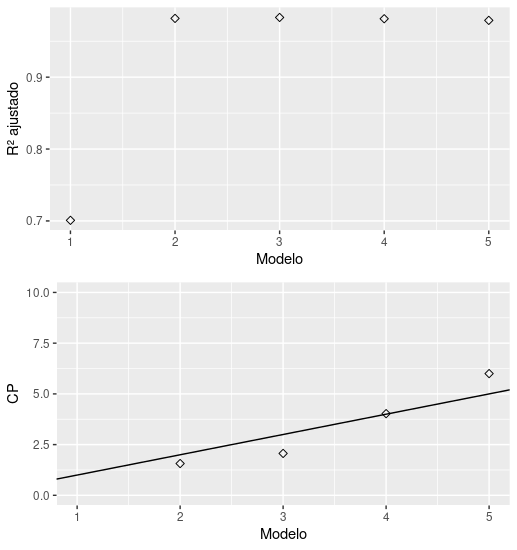
\includegraphics[width=1\textwidth]{resources/Forward.png}
        \end{figure}
    \end{minipage}
\end{minipage}

Del gráfico de la derecha, podemos ver que para el modelo con 4 variables se obtiene el índice de CP que mejor ajusta en la recta identidad.\\
Además, podemos observar que, para ese mismo modelo, el coeficiente de $R^2_{adj}$ es cercano a 1.\\
Por lo que finalmente nos quedaríamos con el modelo de 4 variables, siendo la regresión lineal la siguiente:
\begin{equation}\tag{M3}
    Y = 56.43 - 0.27 \cdot X_1 + 1.47 \cdot X_2 + 0.73 \cdot X_3 - 0.22 \cdot X_5
\end{equation}




\hypertarget{ej6}{\subsection*{Ejercicio 6}}
Para los tres modelos planteados en el trabajo práctico estimaremos el error cuadrático medio utilizando el método de resampleo: Leave One Out Cross Validation, obtuvimos los siguientes resultados.

\begin{center}
    \begin{tabular}{|c|c|}
        \hline
        Modelo & $\hat{ECM}$ \\ \hline
        M1 & $21.39$ \\ \hline
        M2 & $14.34$ \\ \hline
        M3 & $15.05$ \\ \hline
    \end{tabular}
\end{center}
De la tabla podemos ver que el modelo que mejor error cuadrático medio obtiene es el modelo 2.
\begin{figure}[H]
    \centering
    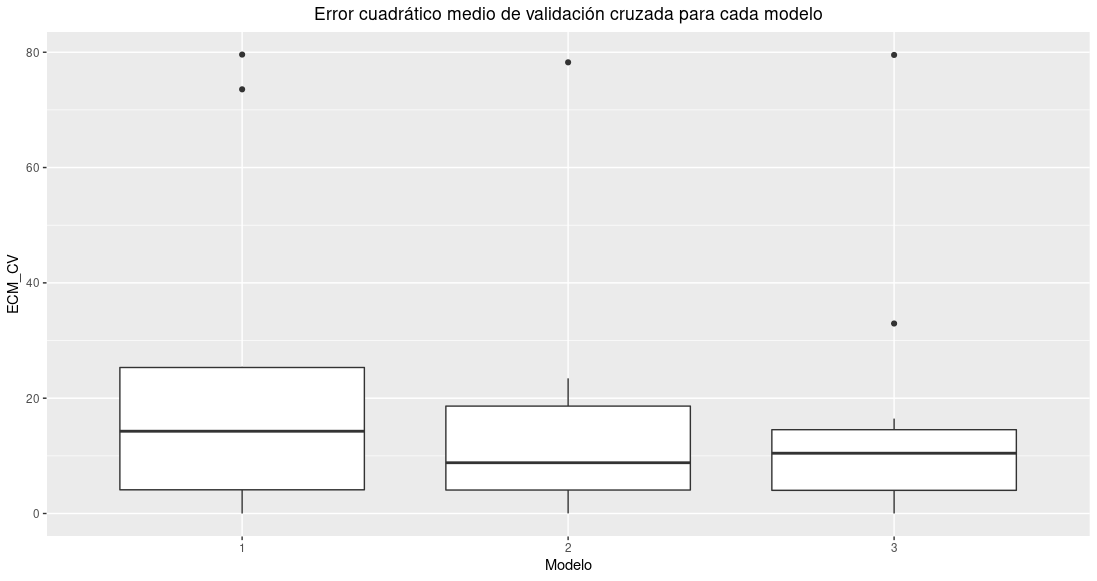
\includegraphics[width=0.8\textwidth]{resources/boxplots_modelos.png}
\end{figure}

En este gráfico en el cual los modelos están ordenados descendentemente por complejidad, podemos ver sobre el rango intercuartílico como que a medida que la complejidad disminuye lo hace la dispersión. Reconocemos particularmente ambos valores atípicos identificados en el ítem 1, los cuales generan un aumento fuerte en la media de la estimación del error cuadrático medio.
\vskip0.2cm
Siendo que en el ejercicio 5 en los modelos con 2 y 3 variables observamos valores para $R^2_{adj}$ y $CP$ muy parecidos a lo ideal, queremos ver cómo se comportarán estimando el error cuadrático medio con LOOCV:
\begin{equation}\tag{M4}
    Y = 51.14 + 1.71 \cdot X_2 + 0.73 \cdot X_3
\end{equation}

\begin{equation}\tag{M5}
    Y = 55.88 - 0.26 \cdot X_1 + 1.47 \cdot X_2 + 0.73 \cdot X_3
\end{equation}

Para estos obtuvimos los siguientes resultados:

\begin{center}
    \begin{tabular}{|c|c|}
        \hline
        Modelo & $\hat{ECM}$ \\ \hline
        M4 & $8.12$ \\ \hline
        M5 & $11.85$ \\ \hline
    \end{tabular}
\end{center}

Podemos ver que para el modelo M4, aquel que se compone sólo por las covariables $X_2$ y $X_3$ obtuvo el menor ECM de LOOCV. Queremos remarcar de esta regresión lineal que, además de tener un alto $CP$ y un alto $R^2_{adj}$, se corresponde con lo observado en el ítem 1 para los índices de correlación de Pearson. \\Esto es:
entre $X_2$ y $X_3$ el índice de correlación es lo suficientemente bajo como para permitirnos decir que no tienen una relación lineal entre sí. Sin embargo, ambos coeficientes $X_2$ e $Y$ y $X_3$ e $Y$ son de modulo cercano a $1$, por lo que: esto nos indica que las variables $X_2$ y $X_3$ permiten estimar a $Y$ con coeficientes muy significativos y casi sin relación lineal entre sí, y esto teóricamente debería resultar en una buena regresión.
 



\newpage
\subsection*{Extra}\label{extra}
\subsubsection*{Validación de supuestos}
En esta sección comprobaremos que los supuestos necesarios para utilizar la regresión lineal sean o no válidos para los modelos que nos interesan, estos son: M2 y M4
\vskip0.2cm\textbf{Modelo 2}
\begin{itemize}
    \item \textbf{Homocedasticidad}: comprobaremos los supuestos de homocedasticidad graficando $t_i$ vs $\hat{y}_i$
    \begin{figure}[H]
        \centering
        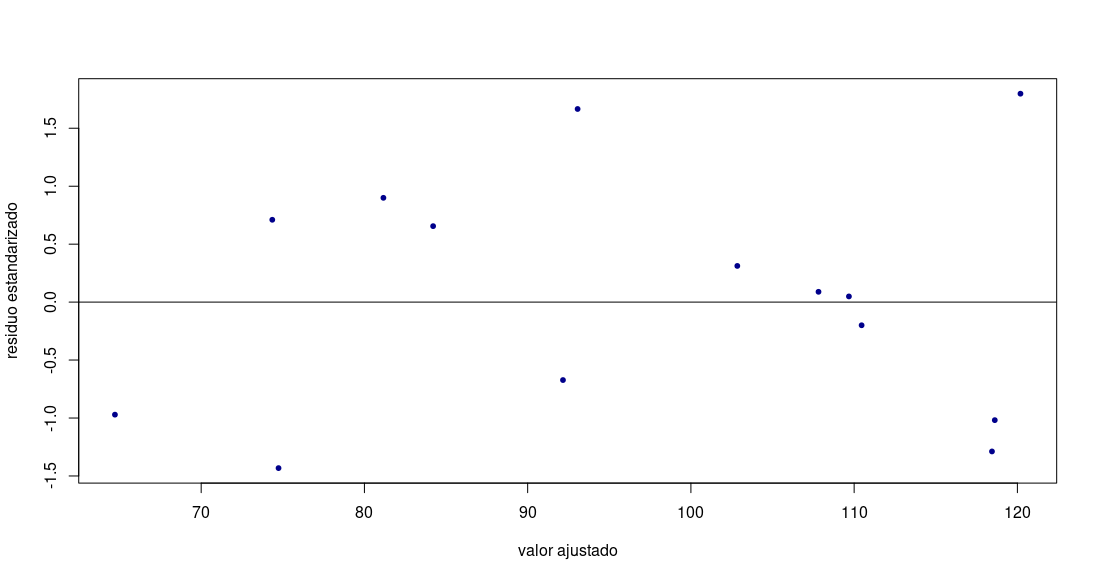
\includegraphics[width=0.7\textwidth]{resources/supuestos_M2.png}
        \caption{Homocedasticidad: modelo 2}
    \end{figure}
    Podemos ver que si bien no aparenta haber una relación de dependencia entre los valores estimados y los residuos, creemos que es difícil obtener esta información con pocas muestras.
    \item \textbf{Normalidad}:
    graficamos un qq-norm para los residuos.
    \begin{figure}[H]
        \centering
        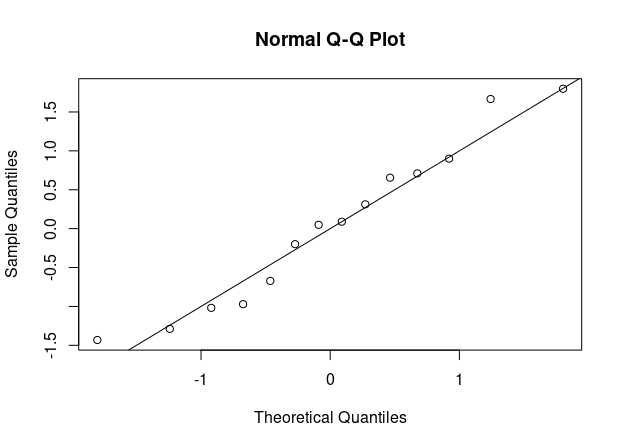
\includegraphics[width=0.7\textwidth]{resources/normalidad_m2.png}
        \caption{Normalidad: modelo 2}
    \end{figure}
    Era de esperarse que estos se distribuyeran aproximadamente como una t de student, y viendo el gráfico no encontramos evidencia suficiente para rechazar dicho supuesto.
\end{itemize}

\vskip0.2cm\textbf{Modelo 4}
\begin{itemize}
    \item \textbf{Homocedasticidad}: comprobaremos los supuestos de homocedasticidad graficando $t_i$ vs $\hat{y}_i$
    \begin{figure}[H]
        \centering
        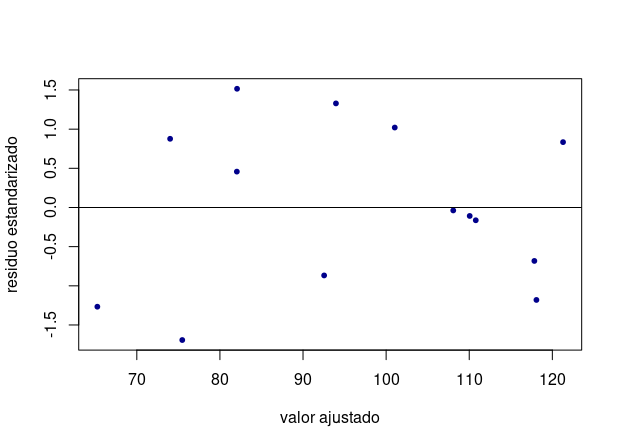
\includegraphics[width=0.7\textwidth]{resources/supuestos_M4.png}
        \caption{Homocedasticidad: modelo 4}
    \end{figure}
    Igual que antes, parece no aparentar ningún tipo de relación muy marcada entre los valores ajustados y los residuos. De todas formas en este caso tampoco tenemos las muestras suficientes como para afirmar o rechazar esta idea.

    \item \textbf{Normalidad}:
    Graficamos un qq-norm para los residuos.
    \begin{figure}[H]
        \centering
        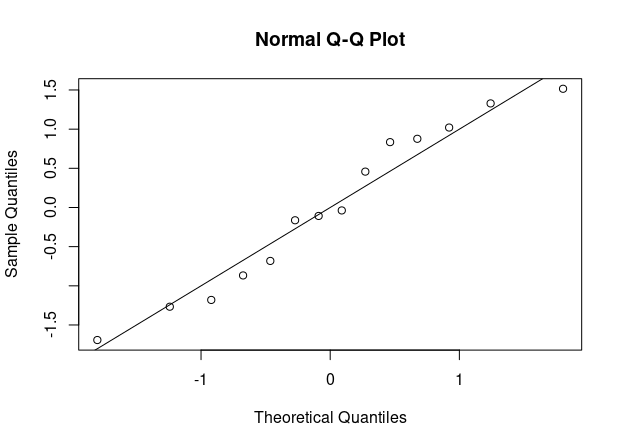
\includegraphics[width=0.7\textwidth]{resources/normalidad_m4.png}
        \caption{Normalidad: modelo 4}
    \end{figure}
    Nuevamente los residuos se distribuyen como esperábamos, esto es: de forma simétrica, similar a una normal pero con las colas pesadas. A diferencia del caso anterior se notan leves protuberancias en los valores intermedios pero no son suficientemente significantes como para decir que no se sigue dicha distribución.
\end{itemize}

\subsubsection*{Gráficos extra}
A continuación graficaremos para el modelo 4 como se ve su estimación en 3 dimensiones.
\begin{figure}[h]
    \centering
    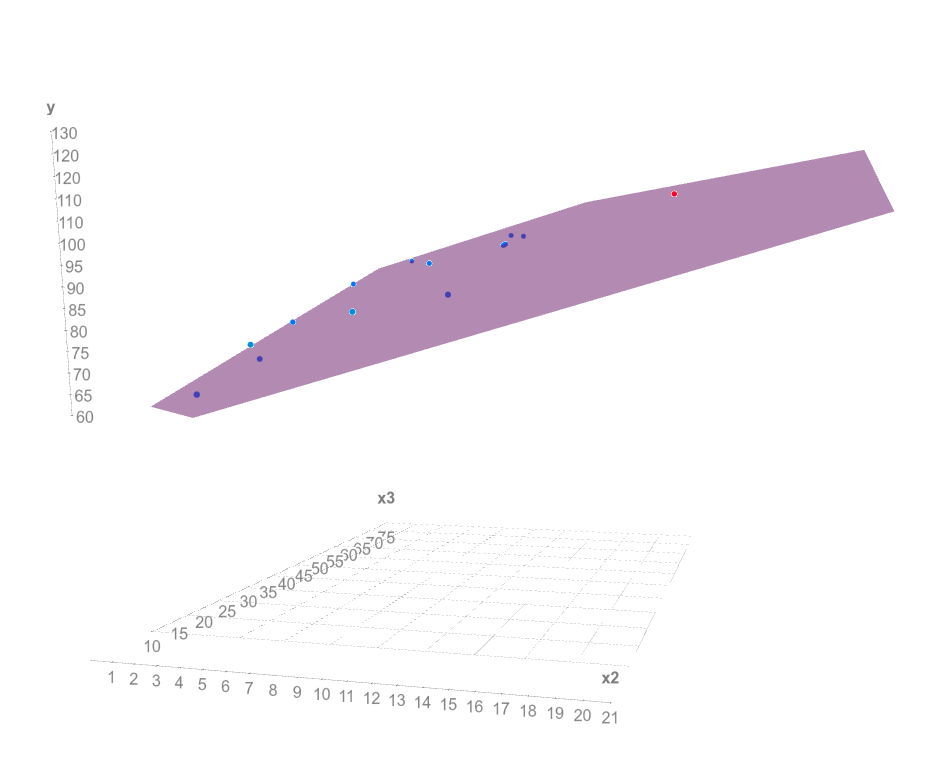
\includegraphics[width=0.8\textwidth]{resources/prediccion_m4.png}
    \caption{Estimación del modelo 4}
\end{figure}

Podemos ver que efectivamente el modelo parece ajustar a las muestras, y parece predecir correctamente.\\
Mostramos en rojo al valor atípico identificado para $X_2$ en la sección 1.

\subsection*{Transformación Box-Cox}
Queremos observar qué sucede si a nuestro modelo 4 le aplicamos una transformación Box-Cox, por lo que primero buscaremos el $\lambda$ de máxima verosimilitud.

\begin{minipage}{\linewidth}
  \begin{minipage}{0.45\linewidth}
    \begin{figure}[H]
        \centering
        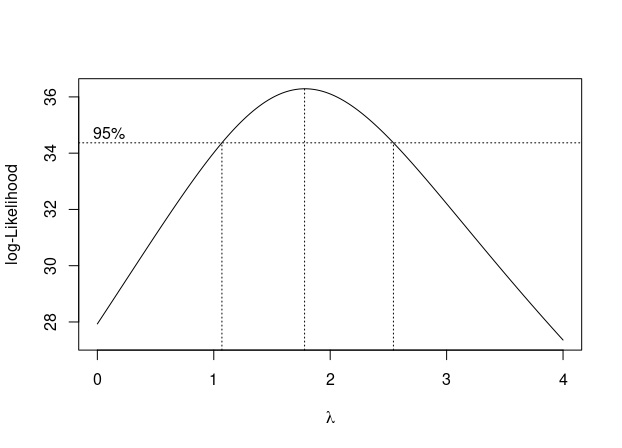
\includegraphics[width=1\textwidth]{resources/lambda_mv.png}
        \caption{Estimación de $\lambda$}
    \end{figure}
  \end{minipage} 
  \begin{minipage}{0.45\linewidth}
    En este gráfico podemos ver:
    \begin{enumerate}
        \item Un intervalo de confianza del $95\%$ para el parámetro $\lambda$, este se mueve en torno al intervalo $[1.1; 2.5]$
        \item El estimador de máxima verosimilitud de $\lambda$ se encuentra en el valor: $1.78$
        \item El valor de $\lambda = 2$ se encuentra dentro del intervalo de confianza del $95\%$
    \end{enumerate}
  \end{minipage}
\end{minipage}

\vskip0.2cm

Para la transformación decidimos utilizar $\lambda = 2$, por lo que, ahora deberíamos regresar el siguiente modelo:
$$
Y^{(2)} = \frac{Y^2 - 1}{2} = \beta_0 + \beta_1 X_2 + \beta_2 X_3
$$
\vskip0.2cm
La regresión que obtuvimos fue la siguiente:
$$\frac{Y^2 - 1}{2} = 614.2  + 167.87 X_2 + 66.14 X_3$$ que es 
equivalente a:
$$Y = \sqrt{1229.4 + 335.74 X_2 + 132.28 X_3}$$

El nuevo modelo planteado obtuvo un error cuadrático medio estimado de $4.02$ que es el mejor de todos.
A continuación mostraremos un gráfico del ajuste propuesto:

\begin{figure}[H]
    \centering
    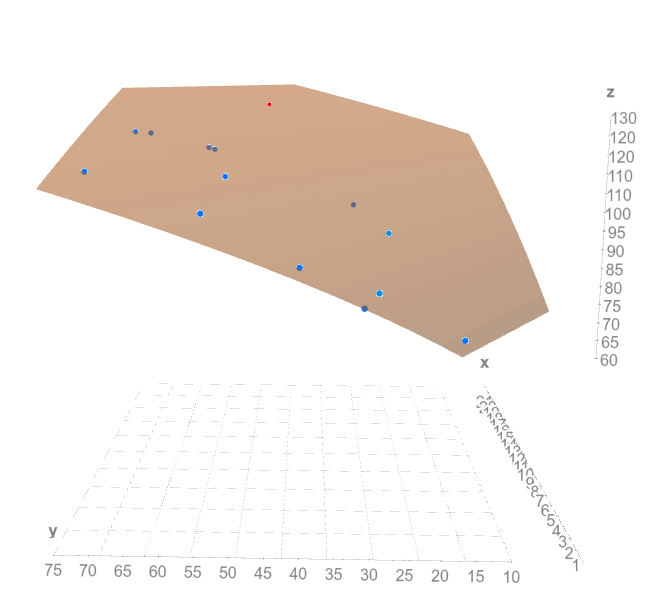
\includegraphics[width=0.7\textwidth]{resources/prediccionfacha.png}
    \caption{Ajuste del modelo transformado}
\end{figure}
\end{document}